\documentclass[aspectratio=169,10pt]{beamer}
\usetheme{Madrid}
\usecolortheme{whale}
\usefonttheme{professionalfonts}

\usepackage[utf8]{inputenc}
\usepackage[T1]{fontenc}
\usepackage[spanish,es-tabla,es-nodecimaldot]{babel}
\usepackage{amsmath,amssymb,amsfonts}
\usepackage{graphicx}
\usepackage{booktabs}
\usepackage{multirow}
\usepackage{array}
\usepackage{xcolor}
\usepackage{hyperref}

\definecolor{uniblue}{RGB}{13, 71, 161}
\definecolor{unidark}{RGB}{10, 37, 64}
\definecolor{unigold}{RGB}{198, 146, 20}
\definecolor{unigreen}{RGB}{27, 94, 32}
\definecolor{unired}{RGB}{183, 28, 28}

\setbeamercolor{palette primary}{bg=unidark,fg=white}
\setbeamercolor{palette secondary}{bg=uniblue,fg=white}
\setbeamercolor{palette tertiary}{bg=unigold,fg=white}
\setbeamercolor{structure}{fg=uniblue}
\setbeamercolor{title}{bg=unidark,fg=white}
\setbeamercolor{frametitle}{bg=unidark,fg=white}
\setbeamercolor{block title}{bg=uniblue,fg=white}
\setbeamercolor{block body}{bg=uniblue!6,fg=black}
\setbeamercolor{block title alerted}{bg=unired,fg=white}
\setbeamercolor{block body alerted}{bg=unired!6,fg=black}
\setbeamercolor{block title example}{bg=unigreen,fg=white}
\setbeamercolor{block body example}{bg=unigreen!6,fg=black}

\setbeamertemplate{navigation symbols}{}
\setbeamertemplate{footline}{
  \leavevmode%
  \hbox{%
  \begin{beamercolorbox}[wd=.30\paperwidth,ht=2.4ex,dp=1ex,center]{author in head/foot}%
    \usebeamerfont{author in head/foot}UNI — Posgrado FIIS (MAE-IA 2026-2)
  \end{beamercolorbox}%
  \begin{beamercolorbox}[wd=.52\paperwidth,ht=2.4ex,dp=1ex,center]{title in head/foot}%
    \usebeamerfont{title in head/foot}Sintonización Evolutiva Robusta NSGA-II en Brazo Robótico 3-DOF (MuJoCo)
  \end{beamercolorbox}%
  \begin{beamercolorbox}[wd=.18\paperwidth,ht=2.4ex,dp=1ex,right]{date in head/foot}%
    \usebeamerfont{date in head/foot}\insertframenumber{} / \inserttotalframenumber\hspace*{2ex}
  \end{beamercolorbox}}%
  \vskip0pt%
}

\title[Control Robótico 3-DOF con NSGA-II]{\textbf{Estrategia Evolutiva Multiobjetivo Elitista (NSGA-II) para la Sintonización Robusta de un Controlador por Torque Computado en un Brazo Robótico Espacial de 3 GDL}}
\subtitle{Asignatura: Computación Evolutiva (2026-2) $\mid$ Docente: Dr. Yván Jesús Túpac Valdivia}
\author[Grupo 2 — MAE-IA UNI]{\textbf{Expositores (3 min c/u):} \\
1. Amit Roy Flores Rivera \quad 2. Franklin Enrique Alegría Barboza \quad 3. Raquel Medianero Huari \\
4. Yasmín Mariela Urrego Montoya \quad 5. José Luis Espinoza Chamaya (\textit{Demo MuJoCo 3D en Vivo})}
\institute[UNI FIIS]{Universidad Nacional de Ingeniería — Facultad de Ingeniería Industrial y de Sistemas\\[0.1cm]
\textbf{Repositorio GitHub:} \url{https://github.com/yasminum/NSGA-II-evol-strategic-multi}}
\date{Lima, Perú — Noviembre 2026}

\begin{document}

% ==============================================================================
% SLIDE 1: PORTADA
% ==============================================================================
\begin{frame}
    \titlepage
\end{frame}

% ==============================================================================
% BLOQUE 1 — EXPOSITOR 1: AMIT ROY FLORES RIVERA (MIN 00:00 - 03:00)
% FASE I: MODELADO DEL PROBLEMA ROBÓTICO Y FORMULACIÓN MULTIOBJETIVO
% ==============================================================================
\begin{frame}{Expositor 1 (Amit Flores): Problema Físico y Falla del Diseño Clásico}
\begin{columns}[T,onlytextwidth]
\begin{column}{0.54\textwidth}
    \begin{block}{1. Dinámica No Lineal Acoplada de Cuerpo Rígido (3-DOF RRR)}
        \vspace{-0.15cm}
        \[
            M(q)\ddot{q} + C(q,\dot{q})\dot{q} + g(q) + f_v\dot{q} + \tau_f(\dot{q}) = \tau + \tau_{\text{ext}}(t)
        \]
        Ley de Control por Torque Computado (CTC) con modelo nominal $(\hat{M}, \hat{h})$:
        \[
            \tau_{\text{cmd}} = \hat{M}(q)\big(\ddot{q}_r + K_p e + K_d \dot{e}\big) + \hat{h}(q,\dot{q})
        \]
    \end{block}
    \begin{alertblock}{2. ¿Por qué fracasa la Asignación Analítica Uniforme ($\omega_n=13, \zeta=1.1$)?}
        \begin{itemize}
            \item \textbf{Asimetría inercial 10:1:} Cintura AX-18A ($m_1=0.25\text{ kg}$, toda la cadena) vs. Hombro en voladizo vs. Codo distal AX-12A ($\tau_{\max,3}=0.45\text{ N}\cdot\text{m}$).
            \item \textbf{Saturación dura no diferenciable:} $\tau_i = \operatorname{clip}(\tau_{\text{cmd},i}, -\tau_{\max,i}, +\tau_{\max,i})$.
            \item \textbf{Incertidumbre planta-modelo ($\hat{M} \neq M$):} Masa $+25\%/+15\%$ y fricción $+30\%$ destruyen la cancelación lineal exacta.
        \end{itemize}
    \end{alertblock}
\end{column}
\begin{column}{0.44\textwidth}
    \centering
    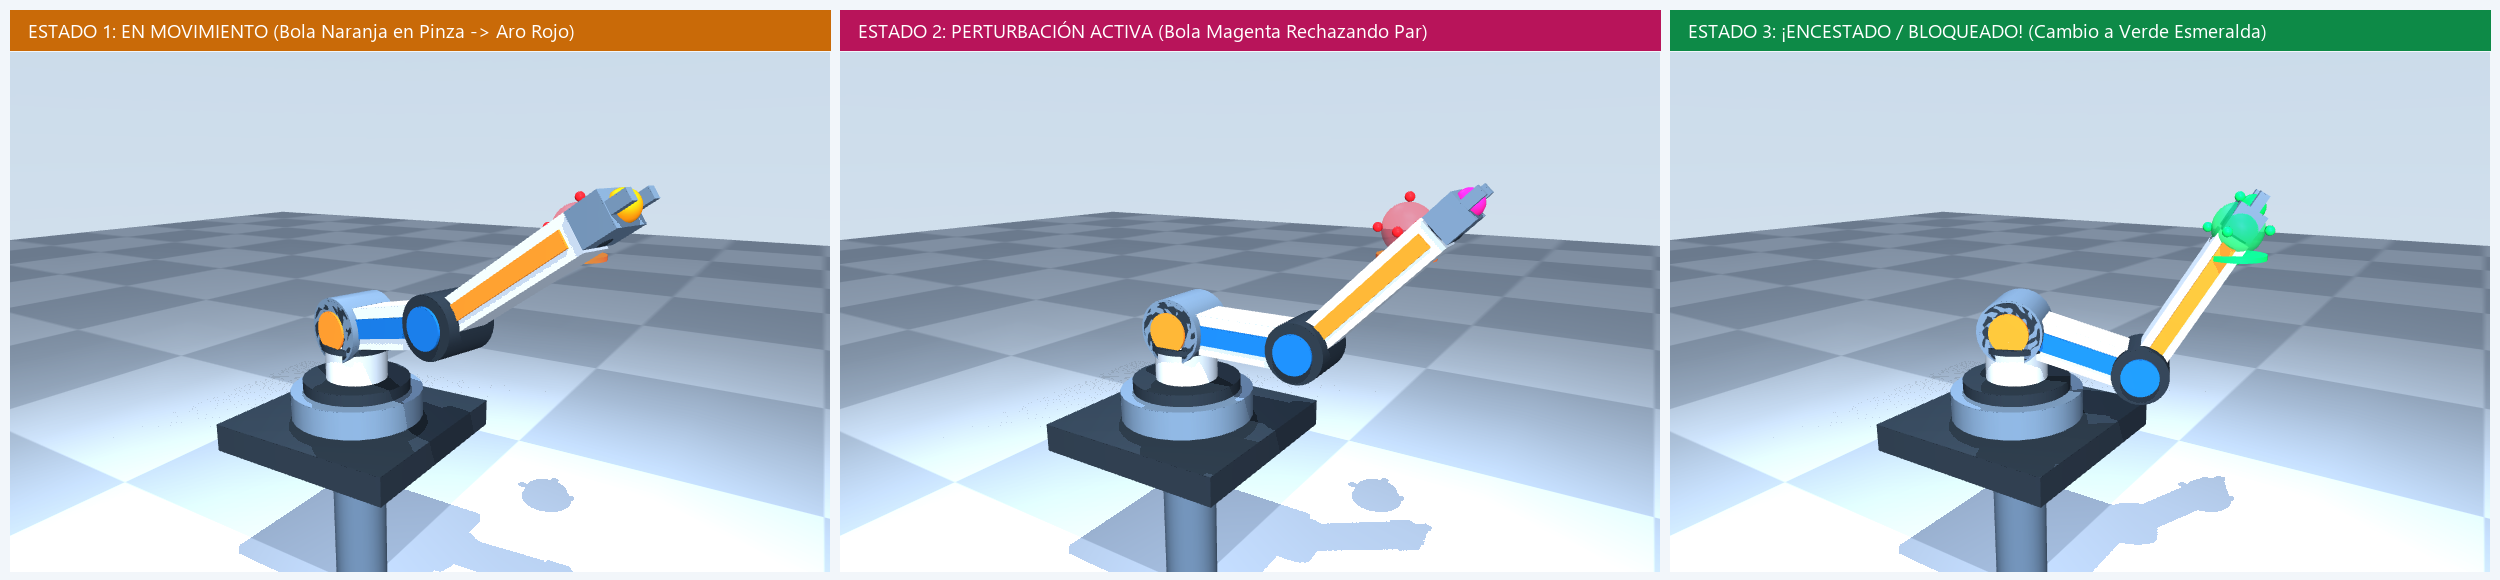
\includegraphics[width=0.98\linewidth]{figuras_ce/fig_estados_3d_enceste.png}
    \vspace{0.05cm}
    {\scriptsize \textbf{Gemelo Digital 3D en MuJoCo ($\Delta t_{\text{sim}}=2\text{ ms}$, Control $100\text{ Hz}$)}: Doble instancia en memoria (Planta Física Perturbada vs. Modelo Nominal $\hat{M}$).}
\end{column}
\end{columns}
\end{frame}

\begin{frame}{Expositor 1 (Amit Flores): Formulación Matemática del Problema Evolutivo}
\begin{columns}[T,onlytextwidth]
\begin{column}{0.52\textwidth}
    \begin{block}{Cromosoma de Decisión ($\theta \in \Omega \subset \mathbb{R}^6$)}
        \[
            \theta = \begin{bmatrix} K_{p1} & K_{p2} & K_{p3} & K_{d1} & K_{d2} & K_{d3} \end{bmatrix}^T
        \]
        \[
            \Omega = [20.0,\, 250.0]^3 \times [3.0,\, 55.0]^3 \subset \mathbb{R}^6
        \]
    \end{block}
    \begin{exampleblock}{4 Escenarios Dinámicos Robustos ($\mathcal{S} = \{s_1,s_2,s_3,s_4\}$, $T=9\text{ s}$)}
        \begin{enumerate}
            \item $s_1$ \textbf{Nominal:} Seguimiento quíntico suave $\mathcal{C}^2$.
            \item $s_2$ \textbf{Perturbación 3D:} Pulso $\tau_{\text{ext}} = [0.035, -0.040, 0.025]^T\text{ N}\cdot\text{m}$ en $t \in [6.0, 6.6]\text{ s}$.
            \item $s_3$ \textbf{Incertidumbre:} $+25\%$ masa eslabón 1, $+15\%$ eslabón 2, $+30\%$ amortiguamiento.
            \item $s_4$ \textbf{Combinado Extremo:} Incertidumbre + Perturbación simultánea.
        \end{enumerate}
    \end{exampleblock}
\end{column}
\begin{column}{0.46\textwidth}
    \begin{block}{Vector Objetivo en Conflicto ($\min_{\theta \in \Omega} \mathbf{F}(\theta)$)}
        \[
            f_1(\theta) = \frac{1}{|\mathcal{S}|}\sum_{s \in \mathcal{S}} \text{RMSE}_{\text{seg}}^{(s)}(\theta) \quad [\text{mm}]
        \]
        \[
            f_2(\theta) = \frac{1}{|\mathcal{S}|}\sum_{s \in \mathcal{S}} \int_0^T \|\tau^{(s)}(t;\theta)\|_2^2\,dt \quad [\text{N}^2\text{m}^2\text{s}]
        \]
        \textbf{+ Extensión Tri-Objetivo Adversarial ($\mathbb{R}^3$):}
        \[
            f_3(\theta) = \int_0^T \|\dot{\tau}(t;\theta)\|_2^2\,dt \quad [\text{N}^2\text{m}^2/\text{s}] \text{ (Anti-Chattering)}
        \]
    \end{block}
    \begin{alertblock}{Restricciones Duras de Hardware}
        $|\tau_i(t)| \le [0.70, 0.70, 0.45]^T\text{ N}\cdot\text{m}$, límites articulares $q_{\min} \le q(t) \le q_{\max}$ y estabilidad finita.
    \end{alertblock}
\end{column}
\end{columns}
\end{frame}

% ==============================================================================
% BLOQUE 2 — EXPOSITOR 2: FRANKLIN ENRIQUE ALEGRÍA BARBOZA (MIN 03:00 - 06:00)
% FASE II Y III: DISEÑO DE NSGA-II, OPERADORES, SELECTOR POST-PARETO Y PARALELIZACIÓN
% ==============================================================================
\begin{frame}{Expositor 2 (Franklin Alegría): Arquitectura Evolutiva NSGA-II y Operadores}
\begin{columns}[T,onlytextwidth]
\begin{column}{0.55\textwidth}
    \begin{block}{¿Por qué NSGA-II con Codificación Real sobre otros Paradigmas?}
        \begin{itemize}
            \item \textbf{Sin pesos arbitrarios a priori:} Descubre la geometría completa del frente de Pareto en una sola corrida pese a la disparidad de escalas ($f_1 \sim 10^1\text{ mm}$ vs. $f_2 \sim 0.5\text{ N}^2\text{m}^2\text{s}$).
            \item \textbf{Operadores continuos libres de Hamming cliffs:}
            \begin{itemize}
                \item \textbf{Cruce SBX ($p_c=0.90, \eta_c=15$):} Poder de búsqueda auto-adaptativo proporcional a $|p_1 - p_2|$.
                \item \textbf{Mutación Polinomial PM ($p_m=1/6, \eta_m=20$):} Modifica 1 gen por cromosoma respetando $\Omega$.
            \end{itemize}
            \item \textbf{Elitismo $(\mu+\lambda)$ + Torneo Aglomerado ($\prec_c$):} Retiene siempre los mejores frentes $\mathcal{F}_1, \mathcal{F}_2$ y maximiza cobertura vía \textit{Crowding Distance}.
        \end{itemize}
    \end{block}
\end{column}
\begin{column}{0.43\textwidth}
    \begin{exampleblock}{Selector Automático Post-Pareto ($\theta^*$)}
        1. Filtra el cono que mejora al controlador base:
        \[
            \mathcal{F}_{\text{dom}} = \{\theta \in \mathcal{F}_1 \mid f_1(\theta) \le f_1(\theta_{\text{base}})\}
        \]
        2. Minimiza la distancia $L_2$ normalizada al punto utópico ideal $z^{\min}$:
        \[
            \theta^* = \arg\min_{\theta \in \mathcal{F}_{\text{dom}}} \sqrt{\sum_{m=1}^2 \left(\frac{f_m(\theta)-z_m^{\min}}{z_m^{\max}-z_m^{\min}}\right)^2}
        \]
    \end{exampleblock}
    \begin{alertblock}{Ingeniería de Software: Speedup $18.7\times$}
        \texttt{ProcessPoolExecutor} (12 núcleos) con modelos MuJoCo pre-cargados en RAM: \textbf{de $1.16\text{ s}$ a $0.062\text{ s}$/eval} ($1,920$ simulaciones en \textbf{$29.88\text{ s}$}).
    \end{alertblock}
\end{column}
\end{columns}
\end{frame}

\begin{frame}{Expositor 2 (Franklin Alegría): Frente de Pareto y Dominancia Estricta}
\begin{columns}[T,onlytextwidth]
\begin{column}{0.56\textwidth}
    \centering
    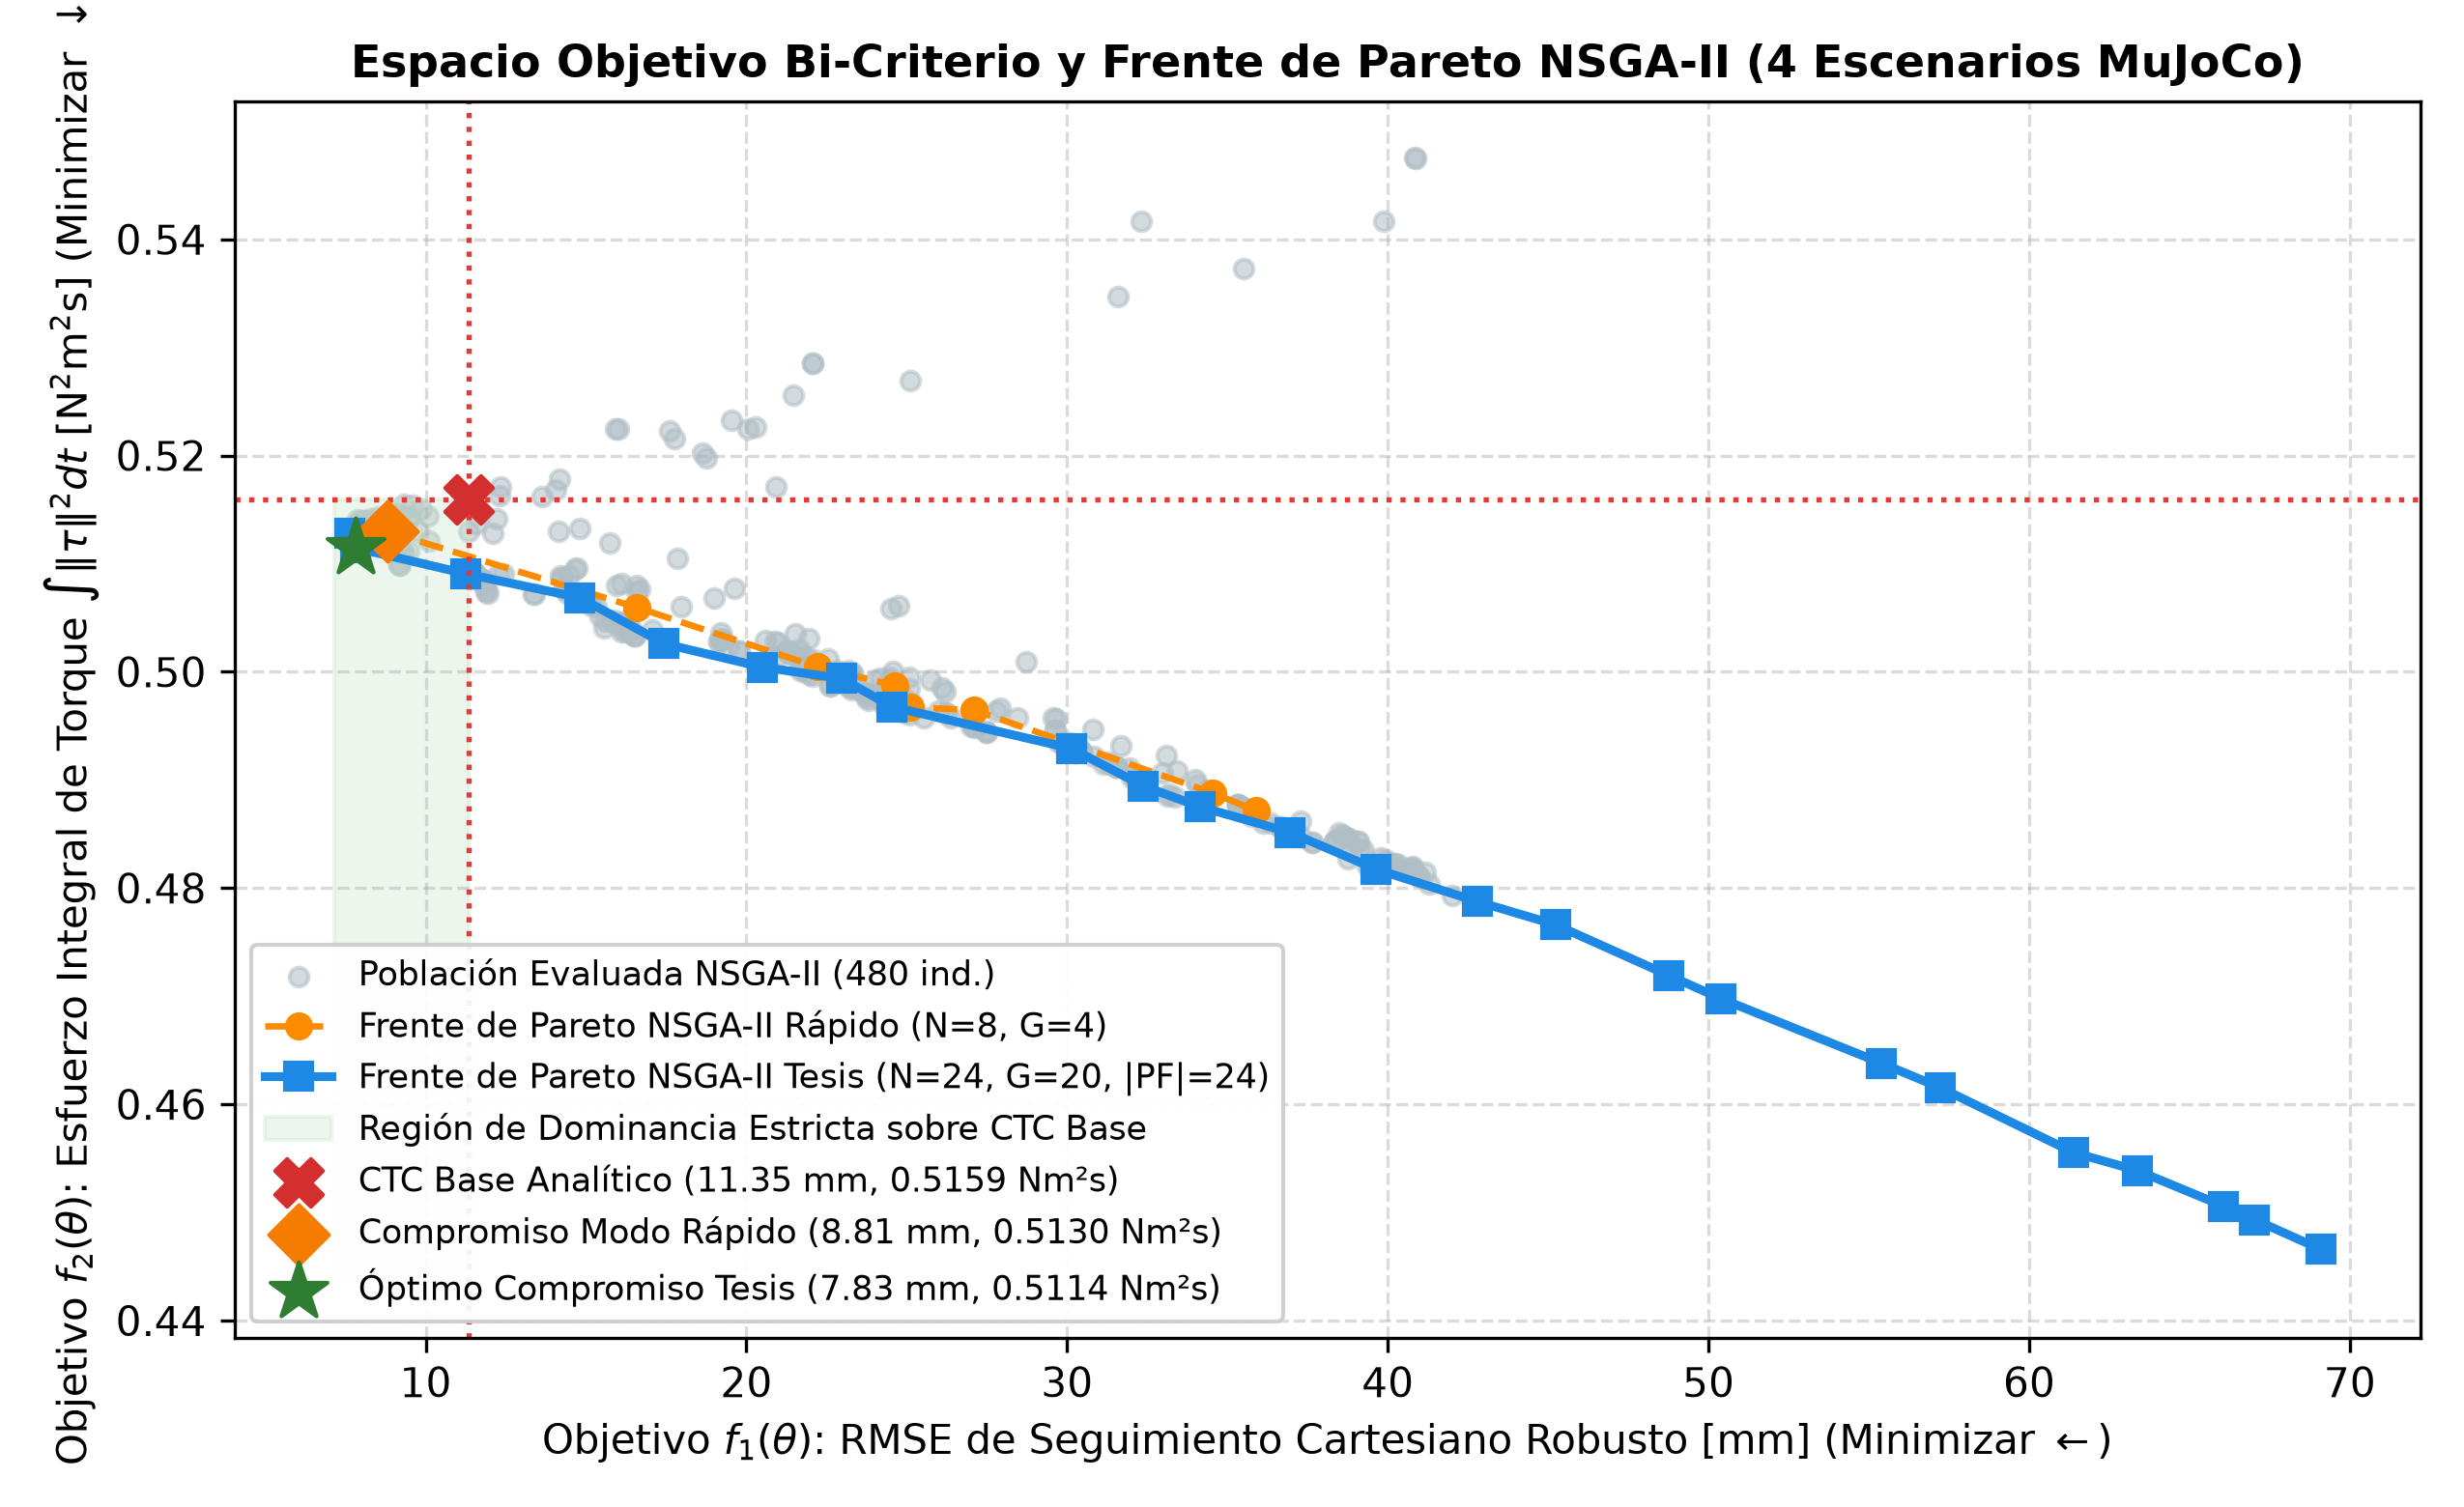
\includegraphics[width=0.99\linewidth]{figuras_ce/fig_ce_01_frente_pareto.png}
\end{column}
\begin{column}{0.42\textwidth}
    \begin{exampleblock}{Dominancia Estricta sobre el Diseño Analítico}
        \begin{itemize}
            \item \textbf{CTC Base ($\omega_n=13, \zeta=1.1$):} $f_1 = 11.353\text{ mm}$, $f_2 = 0.5159\text{ N}^2\text{m}^2\text{s}$.
            \item \textbf{Extremo \#1 (Máx. Precisión):} $f_1 = \mathbf{7.640\text{ mm}}$ ($-32.7\%$), $f_2 = 0.5128$.
            \item \textbf{Compromiso Tesis $\theta^*$ (\#2):} $f_1 = \mathbf{7.827\text{ mm}}$ ($\mathbf{-31.06\%}$), $f_2 = \mathbf{0.5114}$ ($\mathbf{-0.87\%}$).
            \item \textbf{Extremo \#24 (Modo Eco):} $f_2 = \mathbf{0.4466\text{ N}^2\text{m}^2\text{s}}$ ($-13.4\%$ energía).
        \end{itemize}
    \end{exampleblock}
    \begin{block}{Repositorio Abierto Reproducible}
        {\scriptsize \url{https://github.com/yasminum/NSGA-II-evol-strategic-multi}}
    \end{block}
\end{column}
\end{columns}
\end{frame}

% ==============================================================================
% BLOQUE 3 — EXPOSITORA 3: RAQUEL MEDIANERO HUARI (MIN 06:00 - 09:00)
% DINÁMICA POBLACIONAL, HIPERVOLUMEN, SENSIBILIDAD (S1-S9) Y LEY BIOMECÁNICA
% ==============================================================================
\begin{frame}{Expositora 3 (Raquel Medianero): Convergencia, Hipervolumen y Sensibilidad}
\begin{columns}[T,onlytextwidth]
\begin{column}{0.50\textwidth}
    \centering
    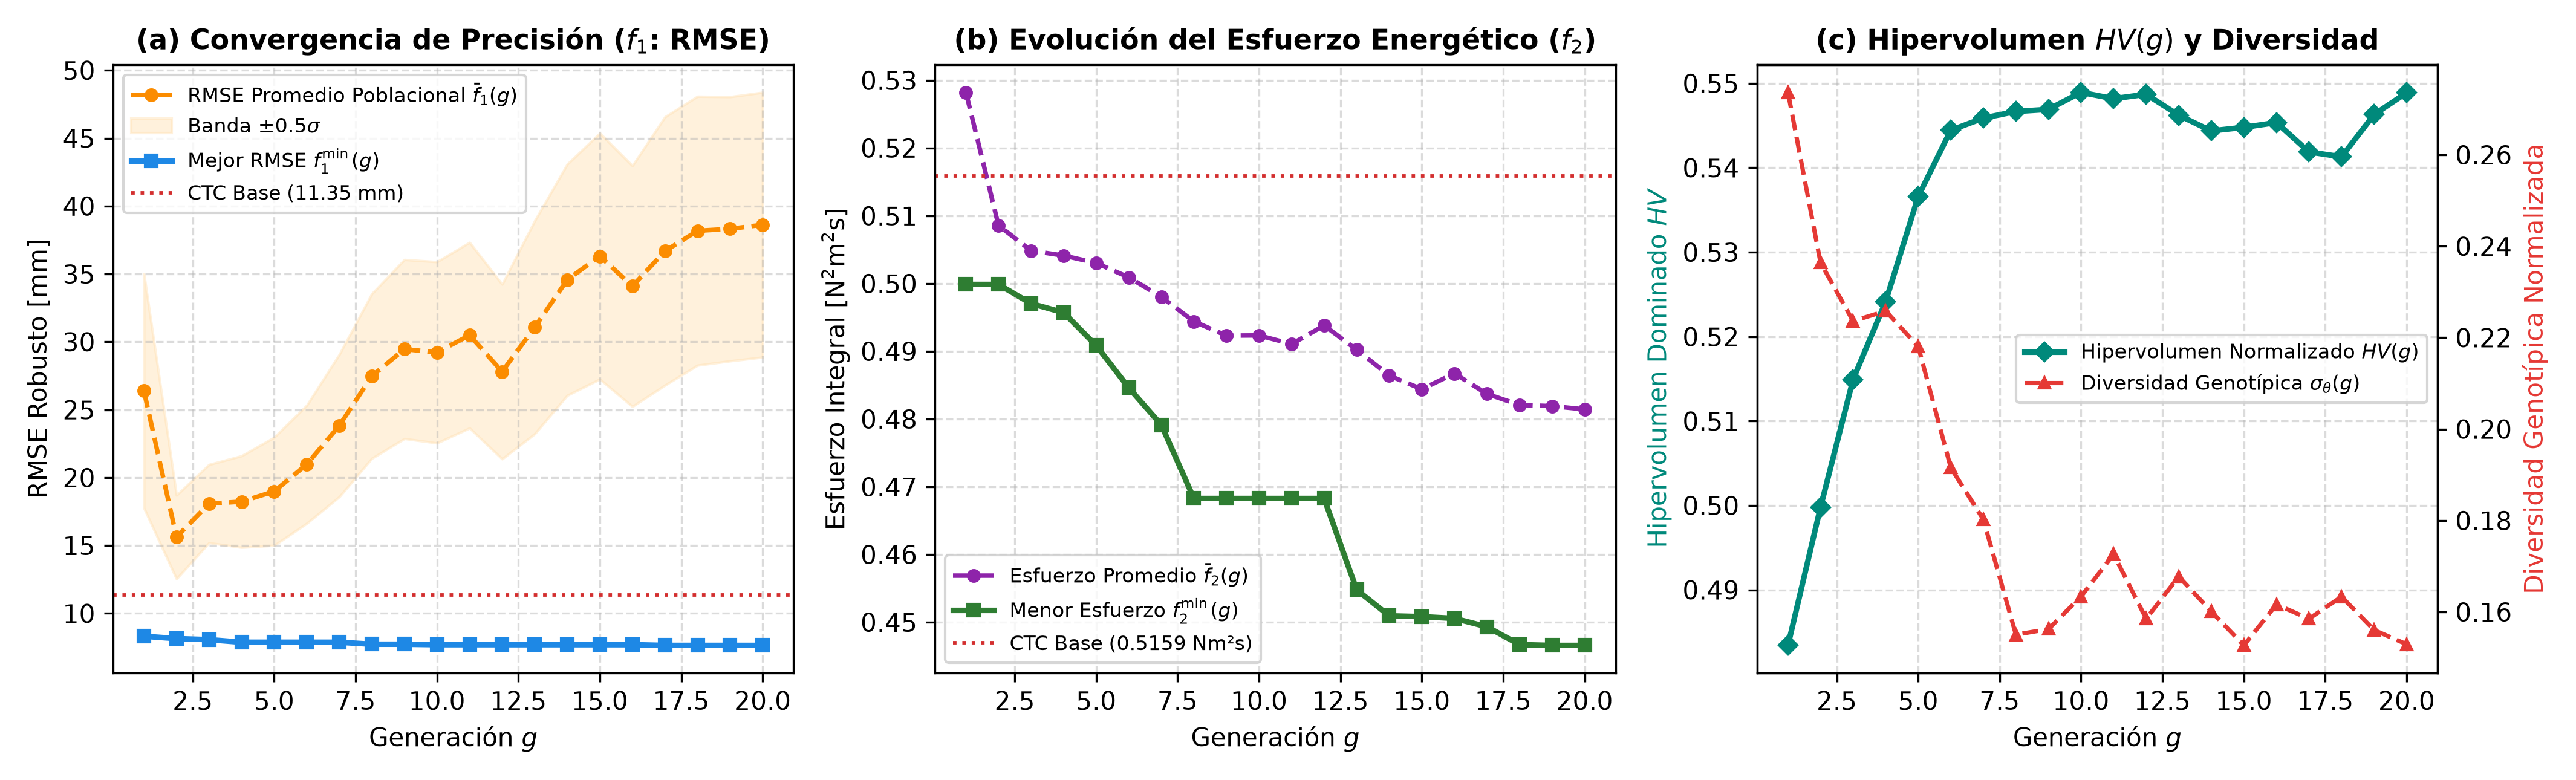
\includegraphics[width=0.99\linewidth]{figuras_ce/fig_ce_02_convergencia_generacional.png}
    \vspace{-0.2cm}
    \begin{block}{\scriptsize Dinámica Generacional ($N_{\text{pop}}=24, G=20$)}
        \scriptsize
        \begin{itemize}
            \item \textbf{Monotonía elitista:} $f_1^{\min}$ baja de $8.316 \to 7.640\text{ mm}$; $f_2^{\min}$ baja de $0.4999 \to 0.4466$.
            \item \textbf{¿Por qué sube $\bar{f}_1(g)$?} \textit{Crowding Distance} puebla la cola de ultra-baja energía ($K_{p2} \in [24,60]$).
            \item \textbf{Sin convergencia prematura:} $HV(g)$ converge a $\mathbf{0.5489}$ con diversidad sana $\sigma_\theta = 0.153 > 0$.
        \end{itemize}
    \end{block}
\end{column}
\begin{column}{0.48\textwidth}
    \centering
    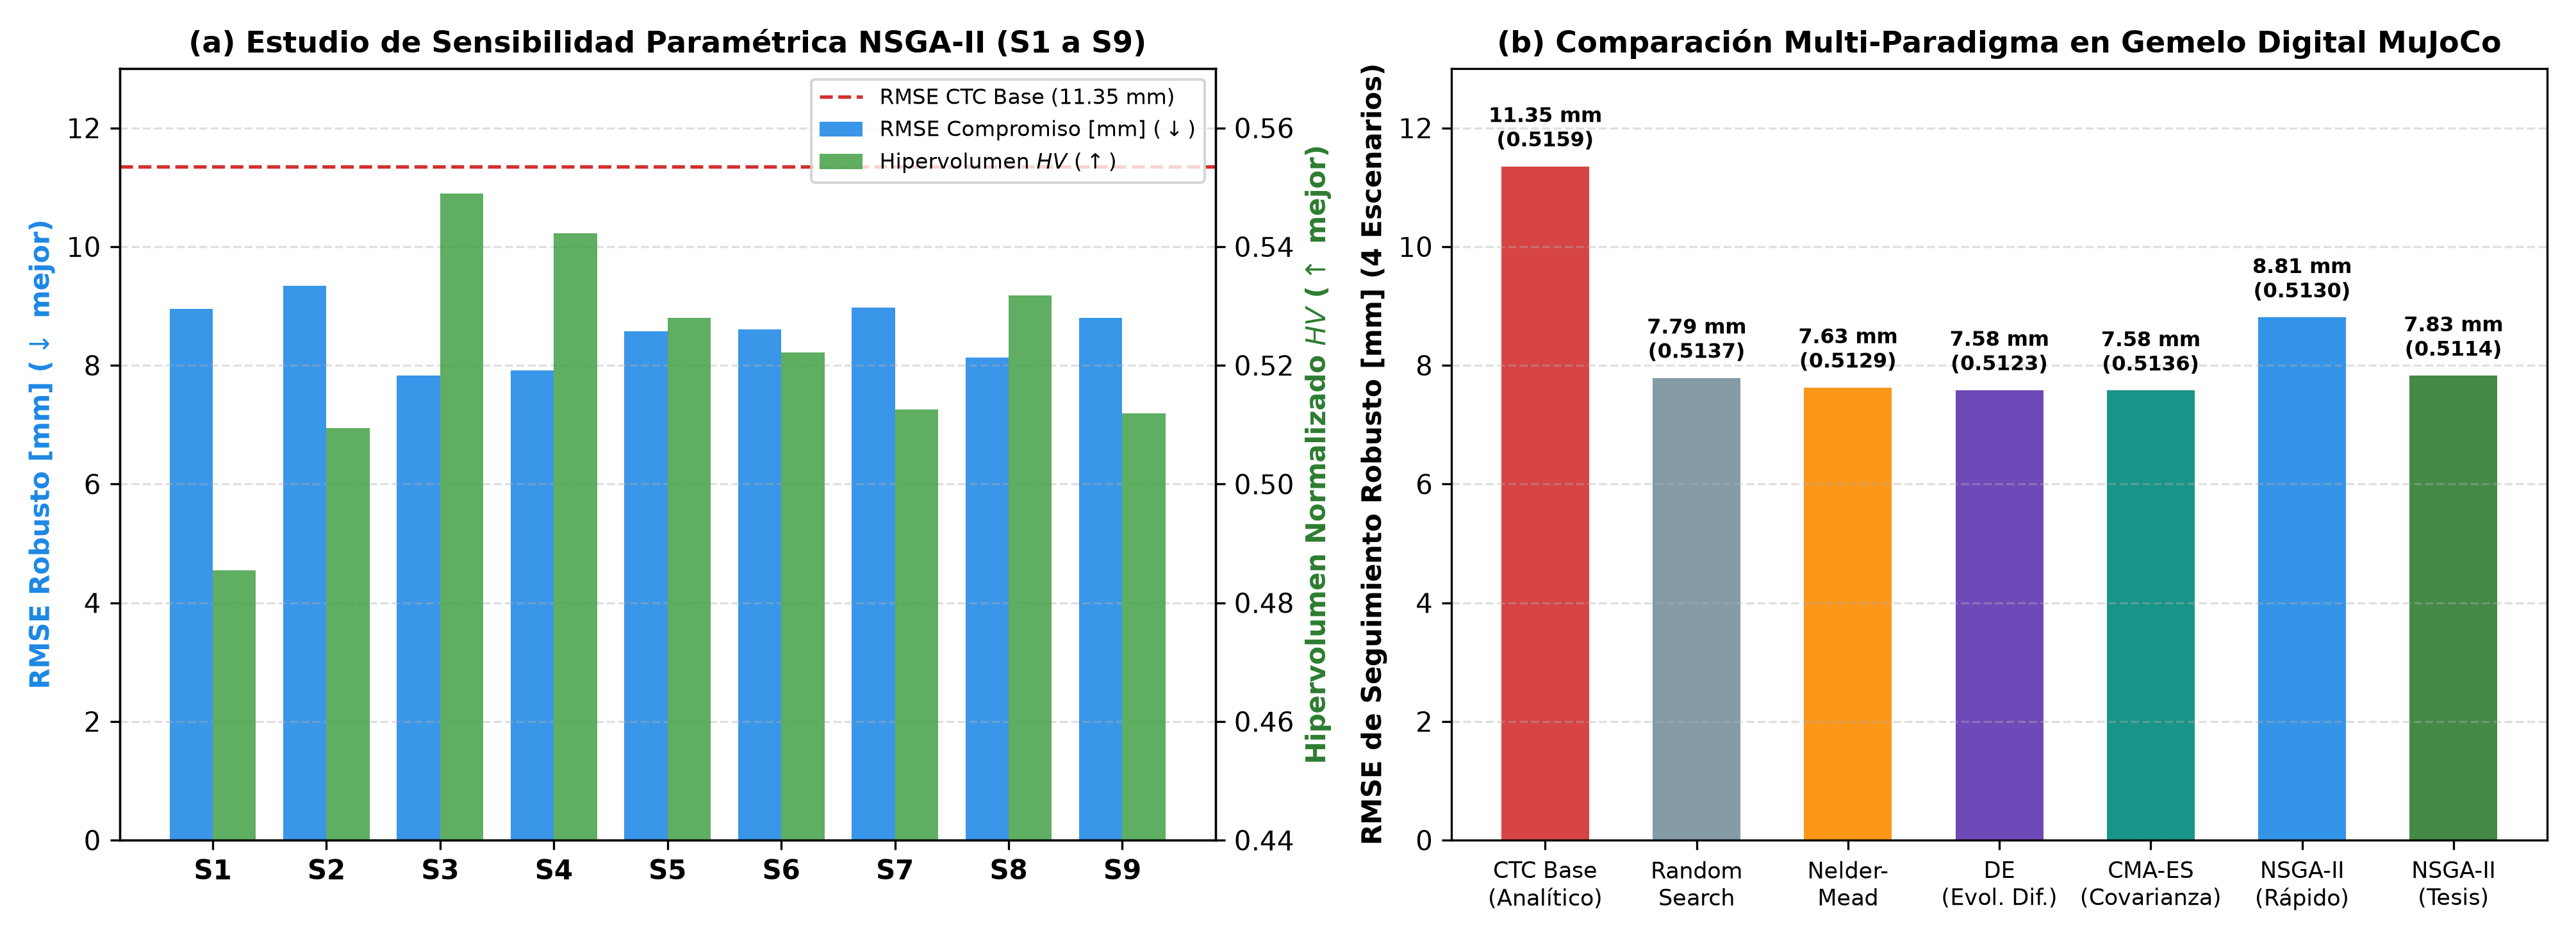
\includegraphics[width=0.99\linewidth]{figuras_ce/fig_ce_03_sensibilidad_y_comparacion.png}
    \vspace{-0.2cm}
    \begin{exampleblock}{\scriptsize Estudio de Sensibilidad ($S_1 \dots S_9$)}
        \scriptsize
        \begin{itemize}
            \item \textbf{Profundidad vs. Anchura:} $S_3$ ($24\times 20=480$ evals, $HV=0.5489$, $29.9\text{ s}$) supera a $S_4$ ($36\times 15=540$ evals, $HV=0.5422$, $37.8\text{ s}$).
            \item \textbf{Mutación:} Muy baja ($S_7, p_m=0.05$) estanca en $8.98\text{ mm}$; agresiva ($S_9, \eta_m=5$) destruye bloques constructores ($8.80\text{ mm}$).
        \end{itemize}
    \end{exampleblock}
\end{column}
\end{columns}
\end{frame}

\begin{frame}{Expositora 3 (Raquel Medianero): Interpretación Biomecánica del Cromosoma $\theta^*$}
\begin{columns}[T,onlytextwidth]
\begin{column}{0.54\textwidth}
    \centering
    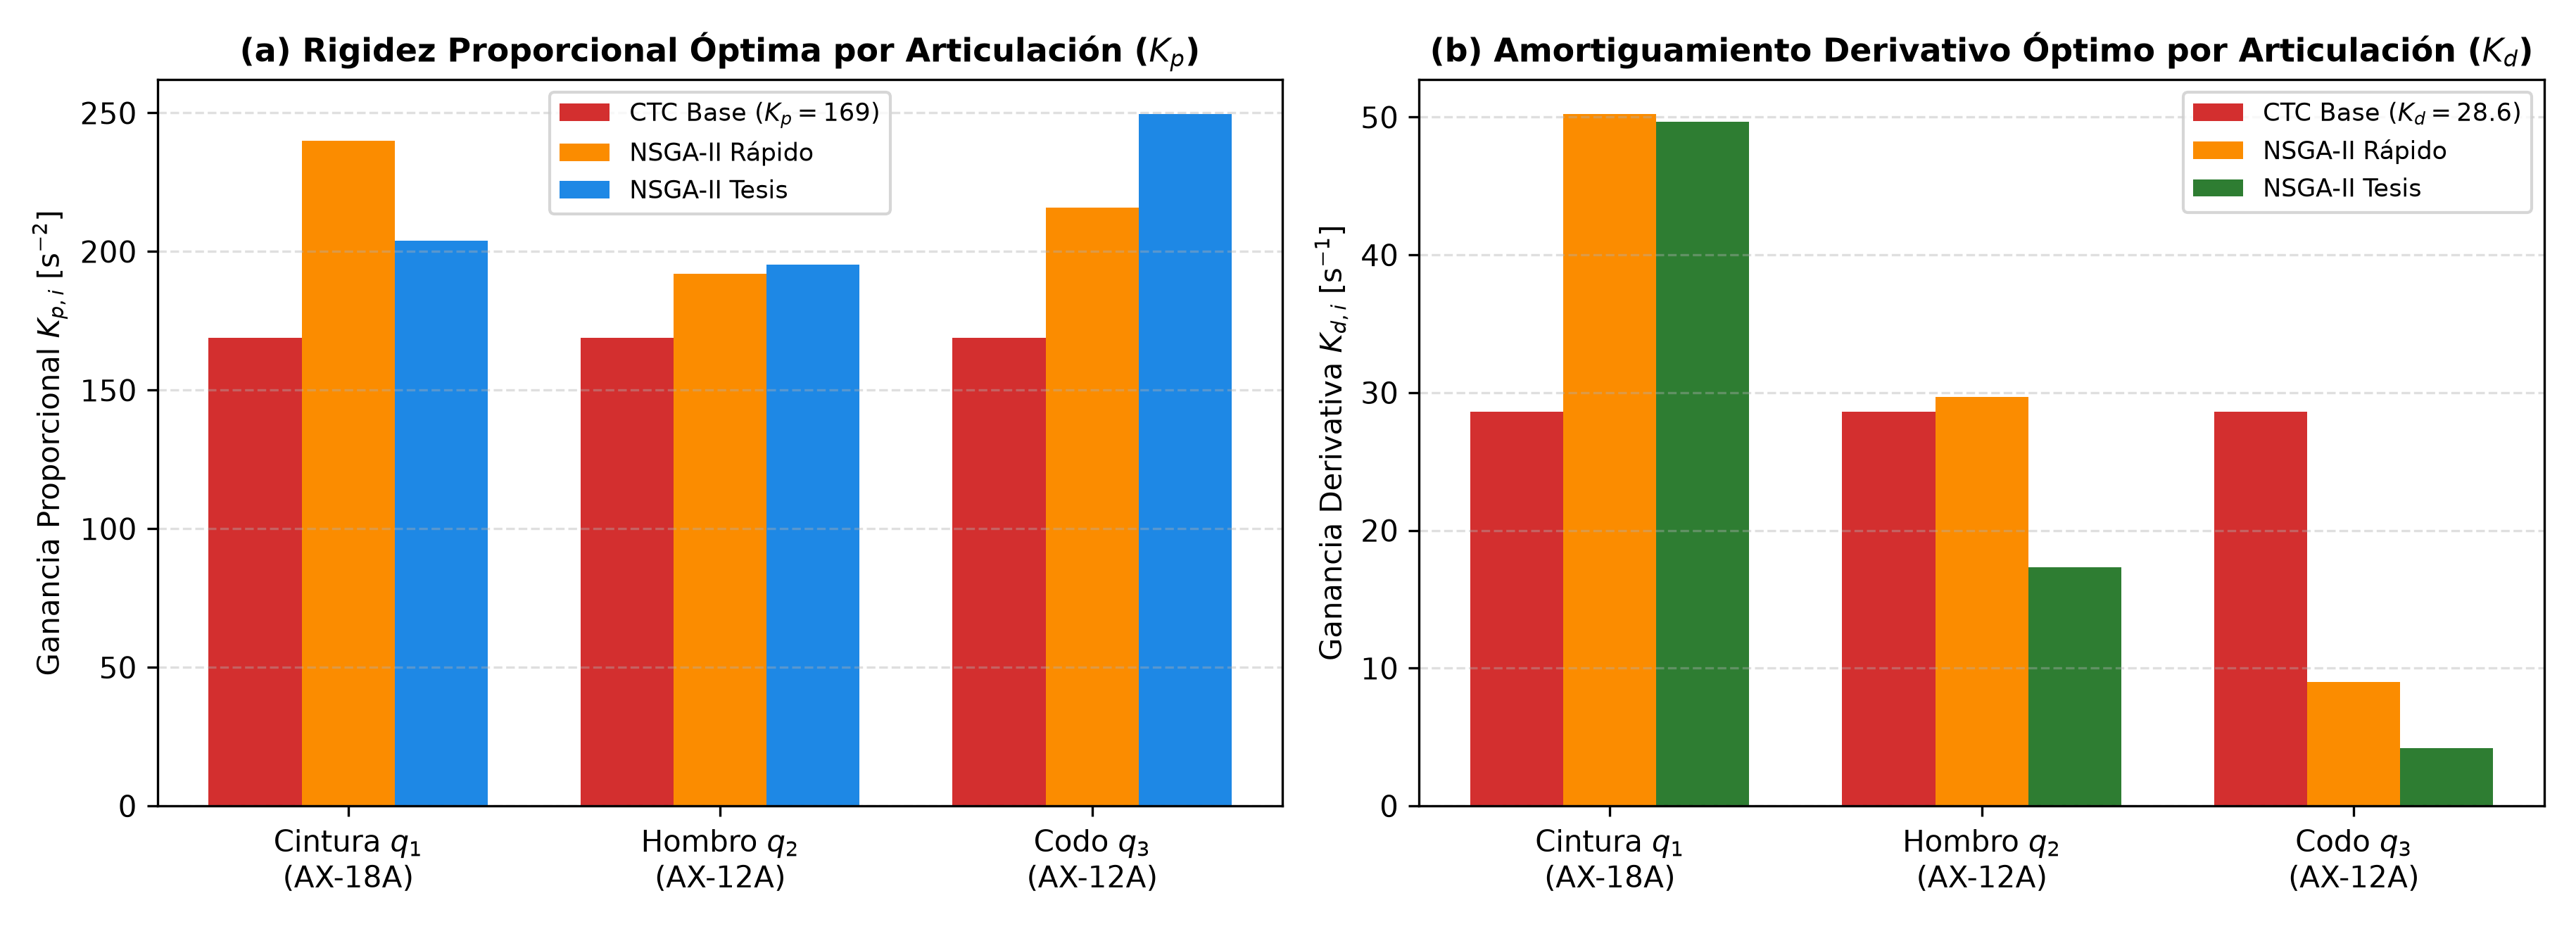
\includegraphics[width=0.99\linewidth]{figuras_ce/fig_ce_04_ganancias_cromosoma.png}
\end{column}
\begin{column}{0.44\textwidth}
    \begin{block}{Ley Estructural Descubierta por NSGA-II}
        \[
            \theta^*_{\text{tesis}} = [203.9,\, 195.4,\, 249.6,\, 49.65,\, 17.33,\, 4.20]^T
        \]
        \begin{enumerate}
            \item \textbf{Rigidización Proporcional ($K_{p,i} > 169$):} Rechaza la incertidumbre de masa $+25\%/+15\%$ y el pulso externo $\tau_{\text{ext}}$.
            \item \textbf{Gradiente Derivativo ($K_{d1} \gg K_{d2} \gg K_{d3}$):}
            \begin{itemize}
                \item Cintura $q_1$: $\zeta_1 \approx 1.74$ (frena la inercia rotacional completa).
                \item Hombro $q_2$: $\zeta_2 \approx 0.62$ (balance gravitacional).
                \item Codo $q_3$: $K_{d3} \to 4.20$ ($\zeta_3 \approx 0.133$), ahorrando par en el actuador de $0.45\text{ N}\cdot\text{m}$.
            \end{itemize}
        \end{enumerate}
    \end{block}
\end{column}
\end{columns}
\end{frame}

% ==============================================================================
% BLOQUE 4 — EXPOSITORA 4: YASMÍN MARIELA URREGO MONTOYA (MIN 09:00 - 12:00)
% BENCHMARK MULTI-PARADIGMA Y CONFRONTACIÓN ADVERSARIAL EN MUJOCO HOSTIL (30 SEMILLAS)
% ==============================================================================
\begin{frame}{Expositora 4 (Yasmín Urrego): Benchmark contra 6 Optimizadores y 5 Controladores}
\begin{columns}[T,onlytextwidth]
\begin{column}{0.52\textwidth}
    \begin{block}{\scriptsize A. Comparación contra Algoritmos de Optimización}
        \scriptsize
        \resizebox{\linewidth}{!}{%
        \begin{tabular}{l c c c c}
        \toprule
        \textbf{Algoritmo} & \textbf{Evals} & \textbf{RMSE [mm]} & \textbf{Esfuerzo} & \textbf{Frente PF} \\
        \midrule
        1. CTC Base Analítico & 1 & 11.3533 & 0.51592 & No \\
        2. Random Search & 160 & 7.7897 & 0.51367 & No \\
        3. Nelder-Mead Simplex & 60 & 7.6265 & 0.51290 & No \\
        4. \texttt{DE/rand/1/bin} & 160 & 7.5830 & 0.51232 & No \\
        5. \textbf{CMA-ES} & 160 & \textbf{7.5763} & 0.51355 & No \\
        6. \textbf{NSGA-II Compromiso} & 480 & 7.8267 & \textbf{0.51145} & \textbf{Sí (24)} \\
        7. \textbf{NSGA-II Extremo \#1} & 480 & \textbf{7.6404} & 0.51279 & \textbf{Sí (24)} \\
        \bottomrule
        \end{tabular}}
    \end{block}
    \begin{exampleblock}{\scriptsize B. Desempeño en Planta a $100\text{ Hz}$ (\texttt{evaluar\_controladores.py})}
        \scriptsize
        \begin{itemize}
            \item \textbf{Costo de inferencia idéntico al PD:} $\mathbf{0.018\text{ ms}}$ ($810\times$ más veloz que MPC de $14.6\text{ ms}$).
            \item \textbf{Seguimiento nominal:} $4.573\text{ mm}$ vs. $6.879\text{ mm}$ ($\mathbf{-33.5\%}$).
            \item \textbf{Recuperación post-impacto:} $\mathbf{0.382\text{ s}}$ vs. $0.582\text{ s}$ ($\mathbf{-34.4\%}$).
        \end{itemize}
    \end{exampleblock}
\end{column}
\begin{column}{0.46\textwidth}
    \centering
    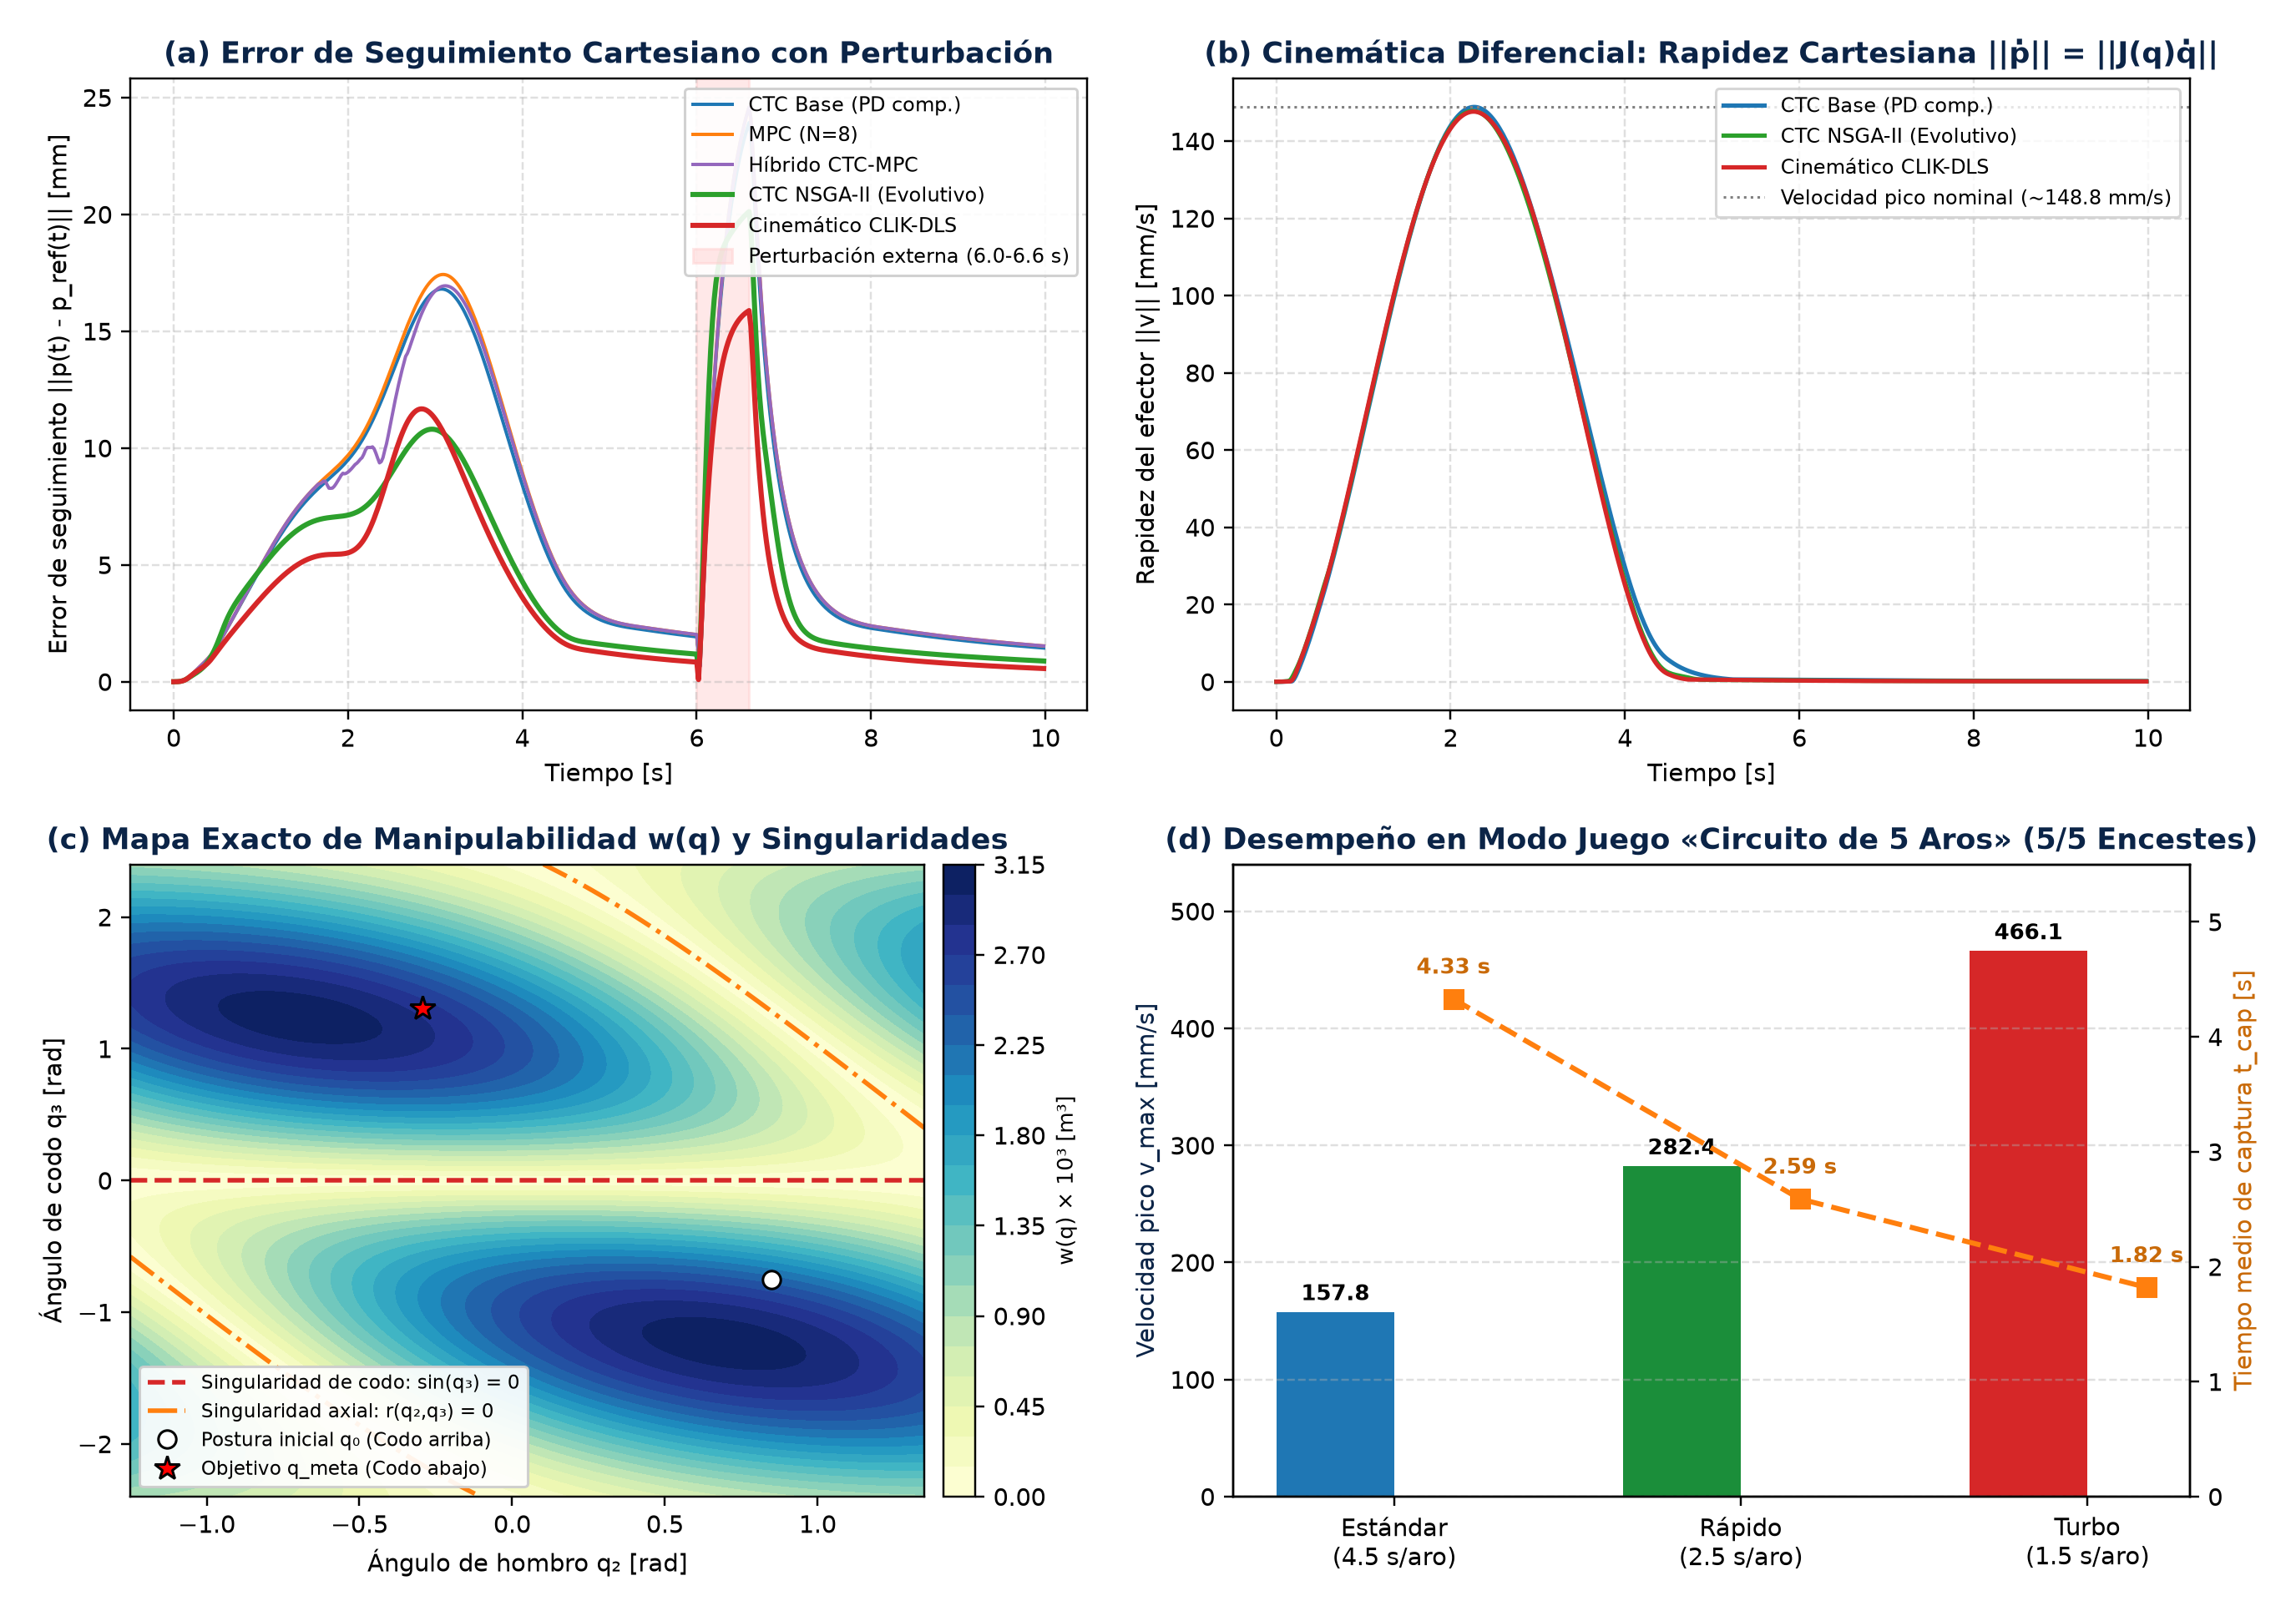
\includegraphics[width=0.99\linewidth]{figuras_ce/fig_curvas_simulacion.png}
\end{column}
\end{columns}
\end{frame}

\begin{frame}{Expositora 4 (Yasmín Urrego): Confrontación Adversarial en Gemelo Hostil ($N=30$)}
\begin{columns}[T,onlytextwidth]
\begin{column}{0.54\textwidth}
    \centering
    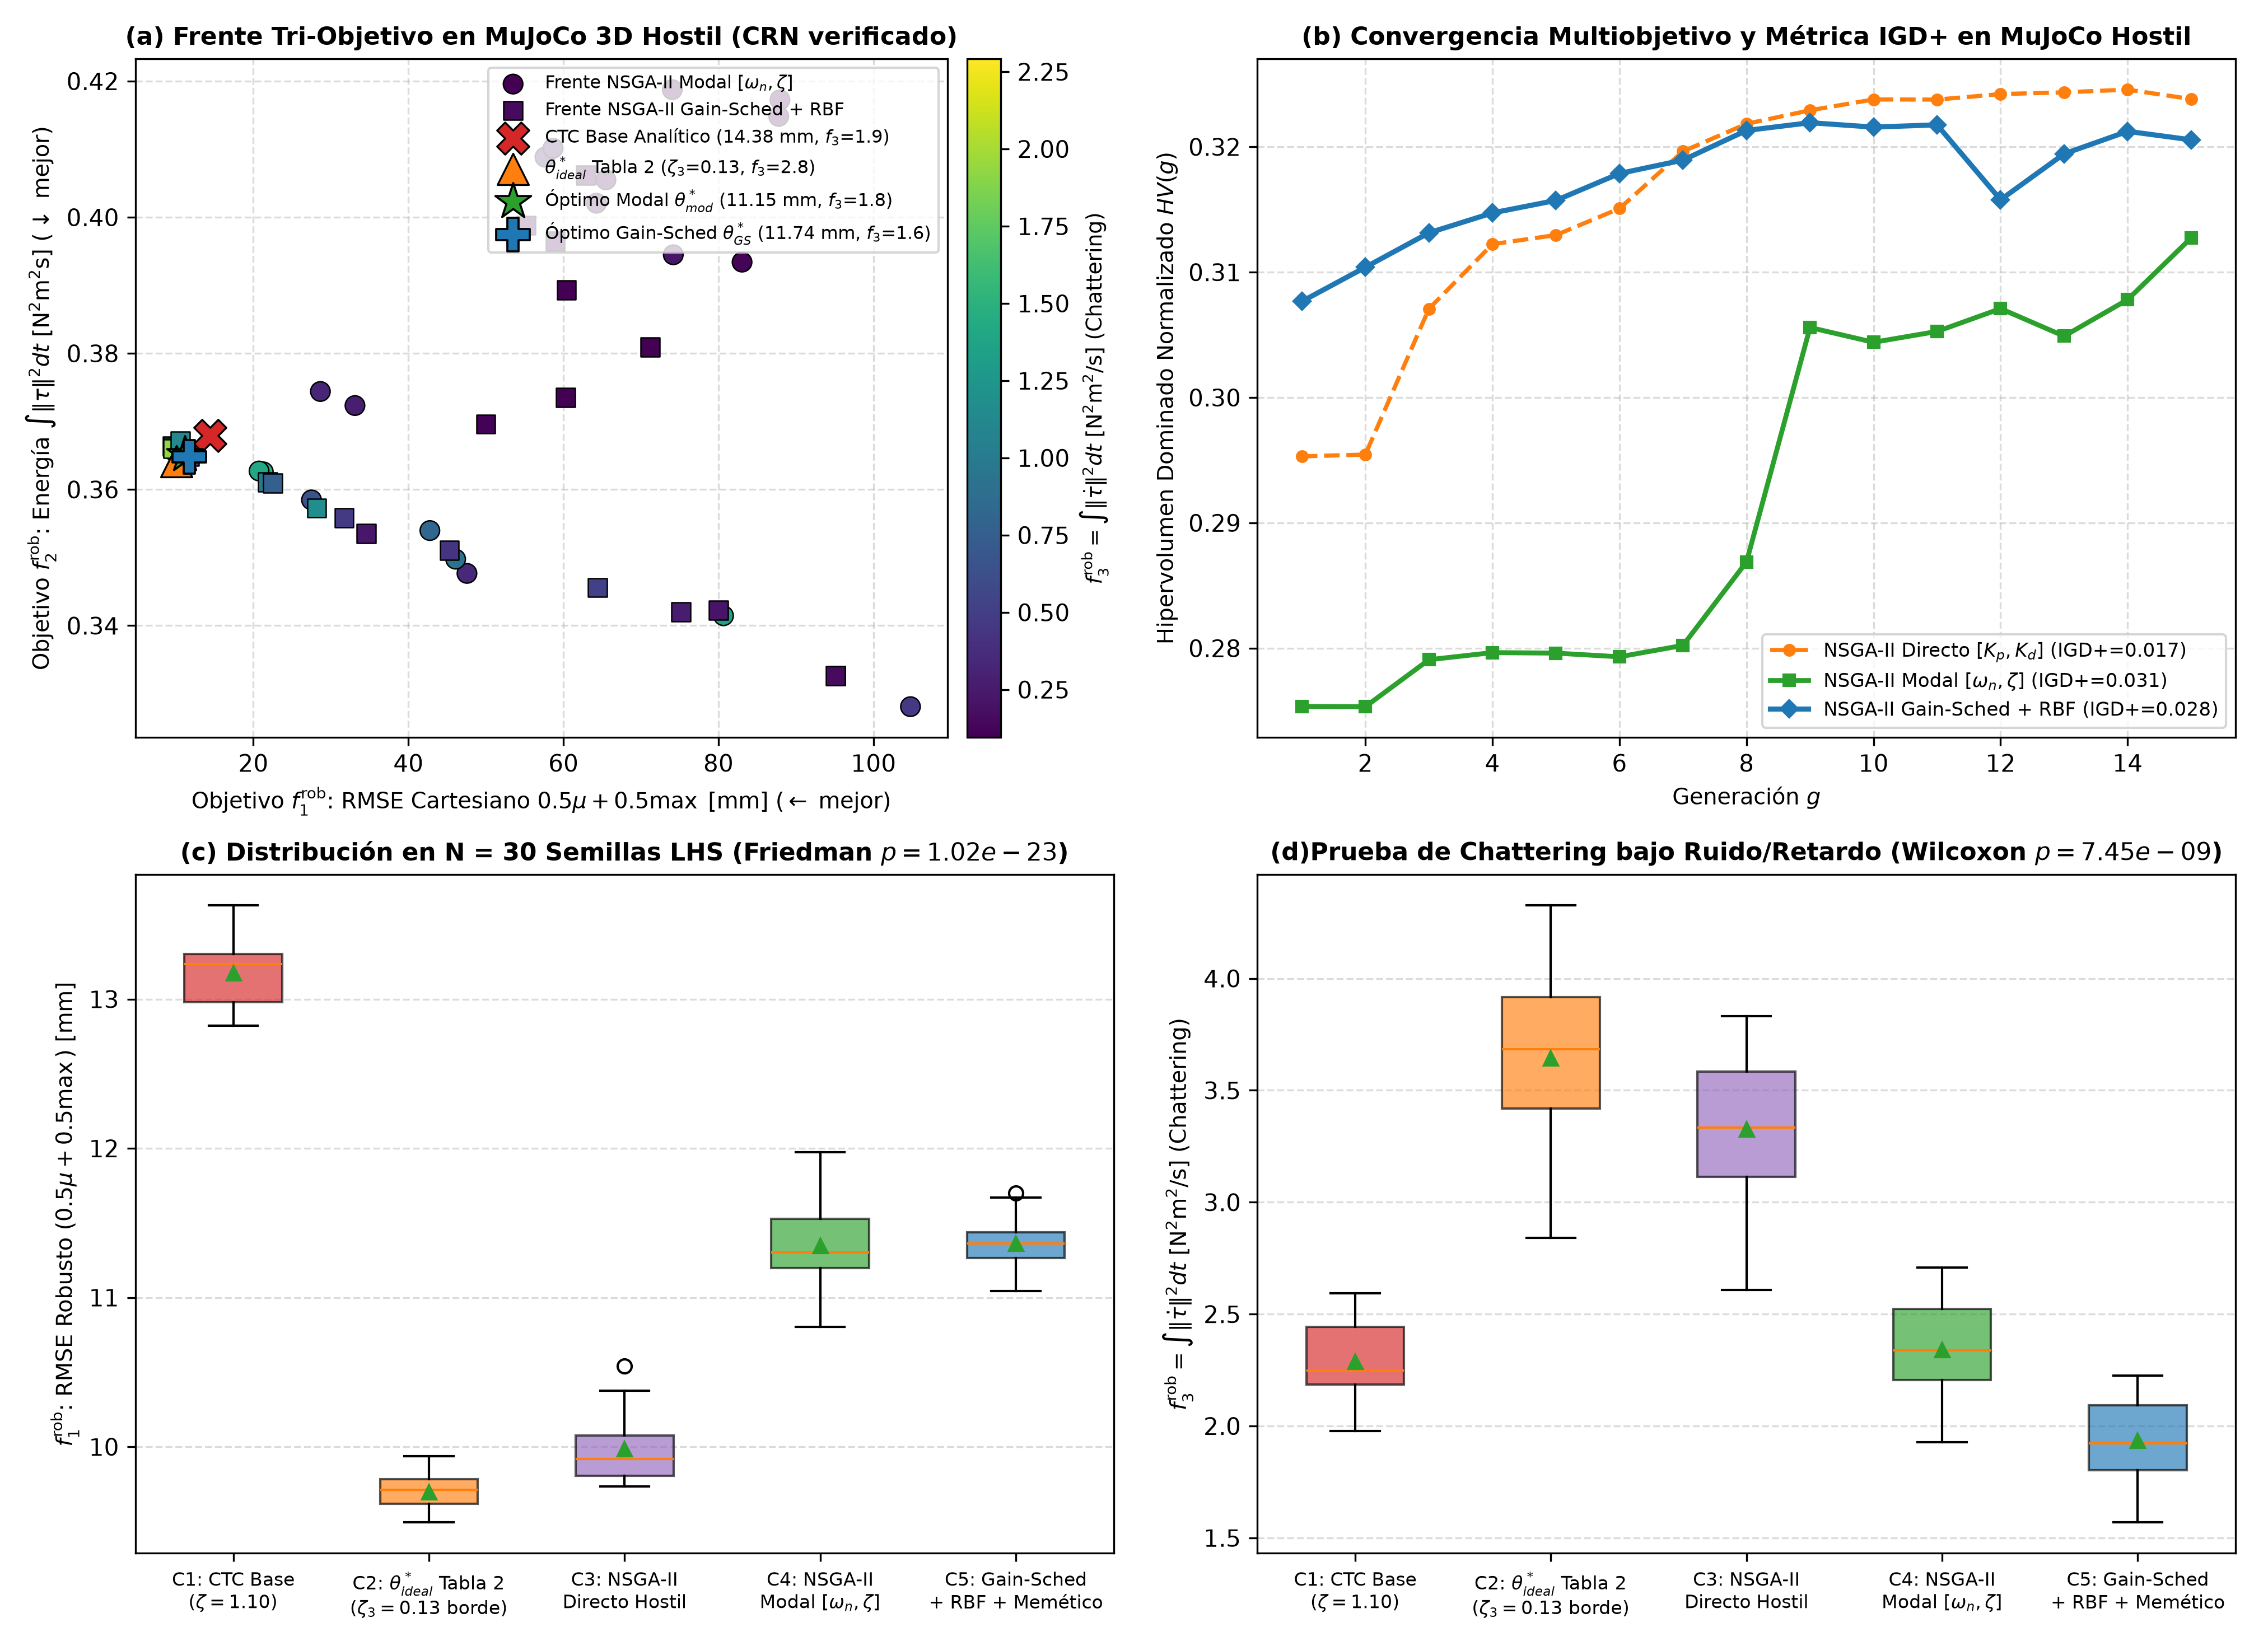
\includegraphics[width=0.99\linewidth]{figuras_ce/fig_ce_05_confrontacion_hostil_30semillas.png}
\end{column}
\begin{column}{0.45\textwidth}
    \begin{alertblock}{\scriptsize Pregunta Científica: ¿Qué pasa con $\zeta_3=0.133$ bajo Ruido y Retardo?}
        \scriptsize
        Gemelo Hostil: Encoder $\sigma_q=0.002\text{ rad}$, Retardo $10\text{ ms}$, Lotes LHS~\cite{mckay1979}, CRN~\cite{law2015}, $0.5\mu + 0.5\max$:
        \begin{itemize}
            \item \textbf{C2 ($\zeta_3=0.133$) amplifica el ruido:} Mantiene $f_1=9.71\text{ mm}$, pero su \textit{chattering} $f_3=\int\|\dot{\tau}\|^2 dt$ explota a $\mathbf{3.684}$ ($\mathbf{+64.0\%}$ peor que el Base, Rango Friedman $5.00$).
        \end{itemize}
    \end{alertblock}
    \begin{exampleblock}{\scriptsize Solución: Genotipo Modal $[\omega_n,\zeta]$ + Gain-Scheduling + RBF}
        \scriptsize
        \resizebox{\linewidth}{!}{%
        \begin{tabular}{l c c c}
        \toprule
        \textbf{Controlador ($N=30$)} & \textbf{$f_1$ [mm]} & \textbf{$f_3$ Chattering} & \textbf{$p_{\text{Holm}}$ ($f_3$)} \\
        \midrule
        C1: CTC Base ($\zeta=1.1$) & 13.235 & 2.247 & $7.45\times 10^{-9}$ \\
        C2: $\theta^*_{\text{ideal}}$ ($\zeta_3=0.133$) & \textbf{9.713} & 3.684 (Peor) & --- \\
        \textbf{C4: Modal $[\omega_n,\zeta]$} & 11.302 & 2.337 ($-36.6\%$) & $7.45\times 10^{-9}$ \\
        \textbf{C5: GS + RBF + Memético} & 11.364 & \textbf{1.922 ($\mathbf{-47.8\%}$)} & $\mathbf{7.45\times 10^{-9}}$ \\
        \bottomrule
        \end{tabular}}
        \vspace{0.05cm}
        \textbf{Friedman ($N=30$):} $p = 6.36 \times 10^{-24}$. \textbf{C5} reduce el \textit{chattering} en $\mathbf{-47.8\%}$ vs. C2 y $\mathbf{-14.5\%}$ vs. C1 Base ($IGD^+=0.0277$).
    \end{exampleblock}
\end{column}
\end{columns}
\end{frame}

% ==============================================================================
% BLOQUE 5 — EXPOSITOR 5: JOSÉ LUIS ESPINOZA CHAMAYA (MIN 12:00 - 15:00)
% DEMOSTRACIÓN EN VIVO DEL GEMELO DIGITAL 3D MUJOCO + CONCLUSIONES Y CIERRE
% ==============================================================================
\begin{frame}{Expositor 5 (José Luis Espinoza): Protocolo de Demostración en Vivo en MuJoCo 3D}
\begin{columns}[T,onlytextwidth]
\begin{column}{0.52\textwidth}
    \begin{block}{Arquitectura Interactiva en Tiempo Real ($500\text{ Hz}$ / $60\text{ FPS}$)}
        Ejecución mediante \texttt{LANZAR\_SIMULADOR\_MUJOCO\_NSGA2.bat}:
        \begin{enumerate}
            \item \textbf{Acto 1 — Captura Sub-milimétrica ($<2.0\text{ mm}$):}
            \begin{itemize}
                \item Carga de $\theta^*$ evolucionado por NSGA-II.
                \item Cambio de esfera a \textcolor{unigreen}{\textbf{Verde Esmeralda}} con error estacionario de $\mathbf{0.068\text{ mm}}$ ($12.2\times$ superior al Base) y $0.0\%$ de saturación.
            \end{itemize}
            \item \textbf{Acto 2 — Inyección de Perturbación Externa 3D en Vivo:}
            \begin{itemize}
                \item Disparo de pulso de torque perturbador en pleno vuelo.
                \item Transición a estado \textcolor{magenta}{\textbf{Magenta}} y recuperación de la zona verde en $\mathbf{0.382\text{ s}}$.
            \end{itemize}
            \item \textbf{Acto 3 — Circuito Autónomo de 5 Aros ($\mathcal{C}^3$ Séptuple):}
            \begin{itemize}
                \item Navegación continua en modos \textbf{Estándar ($3.6\text{ s}$)}, \textbf{Rápido ($2.2\text{ s}$)} y \textbf{Turbo ($1.4\text{ s}$)} con \textbf{5/5 encestes perfectos}.
            \end{itemize}
        \end{enumerate}
    \end{block}
\end{column}
\begin{column}{0.46\textwidth}
    \begin{exampleblock}{Conclusiones, Limitaciones y Líneas Abiertas}
        \scriptsize
        \begin{itemize}
            \item \textbf{Logro 1 (Dominancia Bi-Objetivo):} Reducción de $-31.06\%$ en RMSE robusto y $-33.5\%$ en régimen nominal sin saturar servomotores Dynamixel.
            \item \textbf{Logro 2 (Gemelo Hostil $N=30$):} Reparametrización modal $[\omega_n,\zeta]$ + \textit{Gain-Scheduling} + sustituto RBF suprime el \textit{chattering} en $\mathbf{-47.8\%}$ ($p_{\text{Holm}}=7.45\times 10^{-9}$).
            \item \textbf{Limitación honesta:} El protocolo de $N=30$ semillas certifica la robustez del controlador fijo frente a ruido y trayectorias LHS; medir la varianza entre 30 corridas evolutivas completas queda como extensión.
            \item \textbf{Trabajos Futuros:}
            \begin{enumerate}
                \item \textbf{Coevolución Host--Parasite ($\min\text{--}\max$):} Evolucionar perturbaciones $\tau_{\text{ext}}(t)$ adversarias.
                \item \textbf{NSGA-III en $\mathbb{R}^4$:} Incorporar manipulabilidad $-w_{\min}(q)$.
                \item \textbf{GP / NEAT Residual Sim-to-Real.}
            \end{enumerate}
        \end{itemize}
    \end{exampleblock}
\end{column}
\end{columns}
\end{frame}

\end{document}
